\RequirePackage{pdf14}
\documentclass[aspectratio=169]{beamer}
\mode<presentation>

\hypersetup{pdfpagemode=FullScreen}
\useoutertheme[subsection=false]{smoothbars}

\usepackage[utf8]{inputenc}
\usepackage{tikz}
\usetikzlibrary{shapes}
\usetikzlibrary{arrows.meta}
\usepackage{listings}
\graphicspath{{res/}}

\colorlet{punct}{red!60!black}
\definecolor{delim}{RGB}{20,105,176}

\lstdefinelanguage{json}{%
	basicstyle=\scriptsize\ttfamily,
	showstringspaces=false,
	breaklines=true,
	literate=
		*{:}{{{\color{punct}{:}}}}{1}
		{,}{{{\color{punct}{,}}}}{1}
		{\{}{{{\color{delim}{\{}}}}{1}
		{\}}{{{\color{delim}{\}}}}}{1}
		{[}{{{\color{delim}{[}}}}{1}
		{]}{{{\color{delim}{]}}}}{1}
}

\lstdefinelanguage{caveats}{%
	basicstyle=\scriptsize\ttfamily,
	showstringspaces=false,
	breaklines=true
}

\tikzset{%
	arrow/.style={%
		draw,
		fill=structure.fg,
		single arrow,
		minimum width=5ex,
		minimum height=10ex,
		single arrow head extend=1ex
	}
}
\newcommand{\arrow}{%
\tikz [baseline=-0.5ex]{\node [arrow] {};}
}

\title{\Huge Privay-preserving Systems for Processing Personal Data}
\subtitle{\LARGE DMSN Seminar 2017}
\author{\Large Yousef Amar}
\institute{\includegraphics[height=1cm]{qmul-logo}}
\date{2017-03-14}
\setbeamertemplate{navigation symbols}{}

\begin{document}

\frame{\titlepage}

\begin{frame}
	\frametitle{Background}
	\framesubtitle{What is Personal Data?}
	\begin{columns}[c]
		\column{.7\textwidth}
		\begin{itemize}
			\pause
			\item<2-> Online and social media data
			\begin{itemize}
				\item Facebook, Twitter, Instagram\ldots
				\item Email
				\item Online banking
			\end{itemize}
			\item<3-> Smartphone sensors and wearable
			\begin{itemize}
				\item Message history, GPS, accelerometers, gyroscopes, temperature, microphone, Bluetooth\ldots
				\item Smartwatches, GSR, heart rate, step counter\ldots
			\end{itemize}
			\item<4-> IoT devices in the home
			\begin{itemize}
				\item Smart devices (TVs, fridges, etc)
				\item Lighting, heating, energy usage, proximity sensors\ldots
			\end{itemize}
			\item<5-> Discrete files/blobs/documents vs naturally time series
		\end{itemize}
		\column{.3\textwidth}
		\centering
		
\includegraphics[width=\textwidth]{personal-data}
	\end{columns}
\end{frame}

\begin{frame}
	\frametitle{Background}
	\framesubtitle{The Status Quo}
	\begin{columns}[c]
		\column{.6\textwidth}
		\begin{itemize}
			\item Our digital footprint is explosively increasing
			\item Our data is scattered all over the cloud
			\begin{itemize}
				\item Silos of data inaccessible
				\item Limited analytics; tech and legal bounds
				\item Data breaches on the rise
			\end{itemize}
			\item Cloud solutions, e.g.\ homomorphic encryption face same issues
			\item Most data doesn't even need to leave your home/phone; costs power, bandwidth, latency, and money
			\item Need for different architectural paradigm
		\end{itemize}
		\column{.4\textwidth}
		\centering
		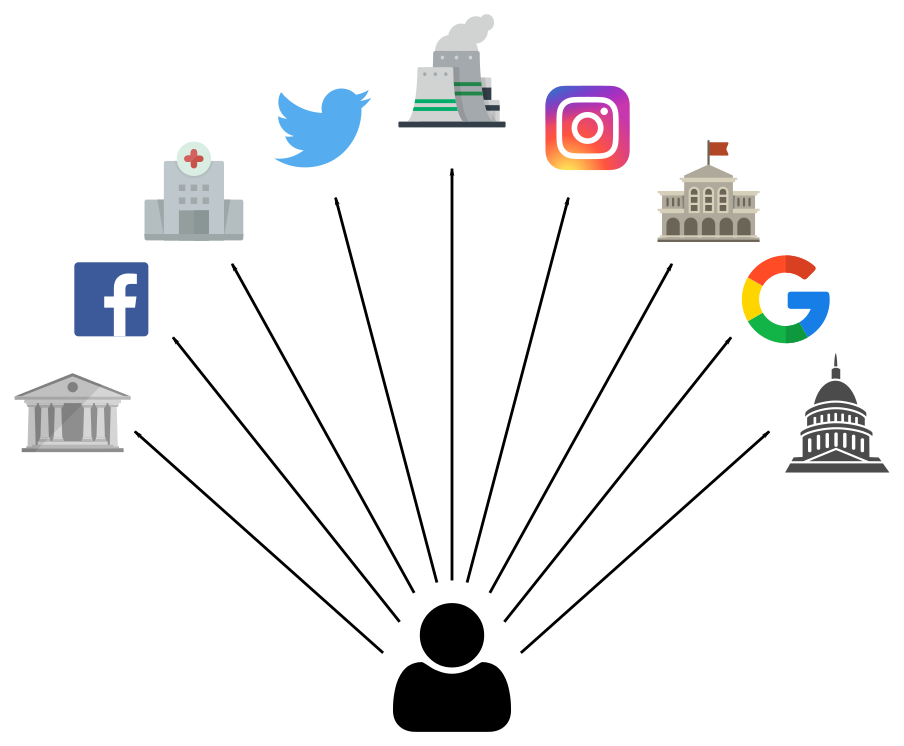
\includegraphics[width=\textwidth]{third-parties}
	\end{columns}
\end{frame}

\begin{frame}
	\frametitle{Background}
	\framesubtitle{Databox}
	\centering
	\includegraphics[width=\linewidth]{architecture7}\\
	\pause
	\textit{How can we design safe, scalable access control systems\\with arbitrary restrictions in this context?}
\end{frame}

% Containers, HTTPS (verify, encrypt)

\begin{frame}[fragile]
	\frametitle{Inter-container Communication}
	\begin{columns}[c]
		\column{.5\textwidth}
		\begin{itemize}
			\item All communication over HTTPS; certs generated run-time; system root CA
			\item RESTful APIs for all operations
			\item Direct mapping of HTTP methods to CRUD functions
			\item Per-route granular permissions
			\item Network-level isolation additionally
			\item Content Security Policy (CSP) to sandbox UIs
		\end{itemize}
		\column{.5\textwidth}
		\centering
		\tiny
		\begin{lstlisting}[language=json]
{
  "target": "smartphone-store",
  "path": "/accelerometer/ts/latest",
  "method": "POST"
}

{
  "target": "smartphone-store",
  "path": "/(sub|unsub)/gps/*",
  "method": "GET"
}
		\end{lstlisting}
	\end{columns}
\end{frame}

\begin{frame}
	\frametitle{Delegated Authorisation}
	\begin{itemize}
		\item Data can be protected through basic authentication; not granular enough
		\item Many APIs use token-based authorization, e.g.\ OAuth 2.0 (Twitter coursework)
	\end{itemize}
	\centering
	\includegraphics[width=\textheight]{oauth2-web-diagram}
\end{frame}

\begin{frame}[fragile]
	\frametitle{Delegated Authorisation}
	\framesubtitle{Macaroons}
	\begin{columns}[c]
		\column{.6\textwidth}
		\begin{itemize}
			\item Google Research: Macaroons
			\begin{itemize}
				\item A standard similar to signed cookies
				\item Can be attenuated by ``caveats''
				\item Embedded permissions
				\item Minting and verification can be separated through shared secret keys
			\end{itemize}
		\end{itemize}
		\begin{lstlisting}[language=caveats]
    target = smartphone-store
    path = /(sub|unsub)/gps/*
    method = GET
    time < 1489405851417

    target = smartphone-store
    path = /light/ts/range
    method = GET
    startTimestamp >= 1489405234352
    endTimestamp <= 1489405259525
		\end{lstlisting}
		\column{.4\textwidth}
		\centering
		\includegraphics[height=\textwidth]{macaroons}
	\end{columns}
\end{frame}

\begin{frame}
	\frametitle{Resource Discovery}
	\begin{itemize}
		\item API for describing APIs
		\item Directory servers
		\item Many competing standards
		\begin{itemize}
			\item Resource Description Framework (RDF)
			\item Web Application Description Language (WADL)
			\item Web Services Description Language (WSDL)
			\item eXtensible Resource Descriptor (XRD)
		\end{itemize}
		\item Subject-predicate-object style pervalent
		\item Different formats and applications --- XML for REST, SOAP, OpenID
	\end{itemize}
\end{frame}

\begin{frame}[fragile]
	\frametitle{Resource Discovery}
	\framesubtitle{Hypercat}
	\begin{columns}[c]
		\column{.49\textwidth}
		\begin{itemize}
			\item Recently joined BSI Group (British Standards Institution)
			\item IoT-first specification design
			\item JSON/REST over XML/SOAP
			\item Only cataloguing; ontologies and authorisation extensible
			\item Discoverability vs accessibility
			\item Catalogues can be nested, allowing decentralisation and distribution
		\end{itemize}
		\column{.51\textwidth}
		\begin{lstlisting}[language=json,basicstyle=\tiny\ttfamily]
{
  "catalogue-metadata": [{
    "rel": "urn:X-hypercat:rels:isContentType",
    "val": "application/vnd.hypercat.catalogue+json"
  }, {
    "rel": "urn:X-hypercat:rels:hasDescription:en",
    "val": "A Databox Store"
  }],
  "items": [{
    "href": "http://some-store/light",
    "item-metadata": [{
      "rel": "urn:X-hypercat:rels:hasDescription:en",
      "val": "Light Datasource"
    }, {
      "rel": "urn:X-databox:rels:hasVendor",
      "val": "Databox Inc."
    }, {
      "rel": "urn:X-databox:rels:isActuator",
      "val": false
    }]
  }]
}
		\end{lstlisting}
	\end{columns}
\end{frame}

\begin{frame}
	\frametitle{Implementation}
	\framesubtitle{Container Relationships}
	\centering
	\includegraphics[width=\textwidth]{relations}
\end{frame}

\begin{frame}
	\frametitle{Implementation}
	\framesubtitle{Authorisation Flow}
	\begin{columns}[c]
		\column{.5\textwidth}
		\centering
		\includegraphics[width=\textwidth]{auth-flow}
		\column{.6\textwidth}
		\begin{enumerate}
			\pause
			\item CM passes unique tokens
			\pause
			\item CM updates permissions
			\pause
			\item Store registers itself
			\pause
			\item Arbiter responds with shared secret
			\pause
			\item Container requests bearer token
			\pause
			\item Arbiter checks and responds
			\pause
			\item Container can now read/write to store
		\end{enumerate}
	\end{columns}
\end{frame}

\begin{frame}[fragile]
	\frametitle{Implementation}
	\framesubtitle{Transcription of Permissions}
	\begin{columns}[c]
		\column{.6\textwidth}
		\begin{enumerate}
			\item Drivers/apps come packaged with a \emph{manifest}
			\begin{itemize}
				\item Contain image metadata
				\item Enumerate granular permissions for sources, concurrency, external access, and hardware
			\end{itemize}
			\item Users generate a Service-level Ageement (SLA)
			\item The arbiter records granted permissions
			\item Tokens are minted based on these
		\end{enumerate}
		\centering
		\vspace{2em}
		\includegraphics[width=0.5\textwidth]{transcription}
		\column{.4\textwidth}
		\centering
		\begin{lstlisting}[language=json]
{
  "name": "app",
  "author": "amar",
  "permissions": [
    {
      "source": "twitter"
      "required": true
    },
    {
      "source": "gps"
    },
    {},
    {}
  ]
}
		\end{lstlisting}
	\end{columns}
\end{frame}

\begin{frame}
	\frametitle{Scalability Evaluation}
	\framesubtitle{Procedure}
	\begin{columns}[c]
		\column{.5\textwidth}
		\centering
		\scriptsize
		\tikzstyle{block} = [rectangle, draw, text width=4em, text centered, minimum height=2em]
		\tikzstyle{store} = [cylinder, shape border rotate=90, draw, text width=4em, text centered, aspect=0.1, minimum height=2em]
		\tikzstyle{line}  = [draw, -{Stealth[length=3mm]}]
		\newcommand{\triplet} {%
			\begin{tikzpicture}[node distance = 8em, auto]
				\node [block] (driver) {Driver};
				\node [store, right of=driver] (store) {Store};
				\node [block, right of=store] (app) {App};
				\path [line] (driver) -- (store);
				\path [line] (store) -- (app);
			\end{tikzpicture}
		}
		\\
		\triplet\\
		\triplet\\
		\triplet\\
		\triplet\\
		$\vdots$

		\pause

		\column{.5\textwidth}
		\centering
		\scriptsize
		\tikzstyle{block} = [rectangle, draw, text width=6em, text centered, minimum height=2em, rounded corners=3pt]
		\tikzstyle{store} = [cylinder, shape border rotate=90, draw, text width=4em, text centered, aspect=0.1, minimum height=2em]
		\tikzstyle{line}  = [draw, -{Stealth[length=3mm]}]
		\newcommand{\pair} {%
			\begin{tikzpicture}[node distance = 10em, auto]
				\node [block] (process) {Stress Tester};
				\node [store, right of=process] (store) {Store};
				\path [line] (process) -- (store);
			\end{tikzpicture}
		}
		\\
		\pair\\
		\pair\\
		\pair\\
		\pair\\
		$\vdots$

	\end{columns}
\end{frame}

\begin{frame}
	\frametitle{Scalability Evaluation}
	\framesubtitle{Results}

	\begin{figure}
		\centering
		\includegraphics[width=0.8\linewidth]{cpu-bins}
		\caption{Percentage CPU Usage by Container Type}
	\end{figure}

	\begin{figure}
		\centering
		\includegraphics[width=0.8\linewidth]{mem-bins}
		\caption{Memory Usage by Container Type}
	\end{figure}
\end{frame}

\begin{frame}
	\frametitle{Scalability Evaluation}
	\framesubtitle{Results}

	\begin{figure}
		\centering
		\includegraphics[width=\linewidth]{io-bins}
		\caption{Sum Net I/O by Container Type}
	\end{figure}
\end{frame}

\begin{frame}
	\frametitle{Scalability Evaluation}
	\framesubtitle{Results}

	\begin{figure}
		\centering
		\includegraphics[width=\linewidth]{stores}
		\caption{Inserts/s over Stores under Maximum Load}
	\end{figure}
\end{frame}

\begin{frame}
	\frametitle{Scalability Evaluation}
	\framesubtitle{Results}

	\begin{figure}
		\centering
		\includegraphics[width=\linewidth]{arbiter}
		\caption{Stores Launched over Time}
	\end{figure}
\end{frame}

\begin{frame}
	\frametitle{Topological Evaluation}
	\framesubtitle{Procedure and Results}

	\begin{columns}[c]
		\column{.4\textwidth}
		Differences in Time to Availability~(TTA)
		\begin{enumerate}
			\item Device $\rightarrow$ Cloud:\\{$65ms$}
			\item Device $\rightarrow$ Cloud $\rightarrow$ Home:\\{$83ms$}
			\item Device $\rightarrow$ Home:\\{$78ms$}
			\item Device $\rightarrow$ Home $\rightarrow$ Cloud:\\{$80ms$}
		\end{enumerate}
		\column{.6\textwidth}
		\begin{figure}
			\centering
			\includegraphics[width=0.7\textwidth]{scenarios}
			\caption{The four possible data flow scenarios tested}
		\end{figure}
	\end{columns}
\end{frame}

\begin{frame}
	\frametitle{Topological Evaluation}
	\framesubtitle{Results}

	\begin{columns}[c]
		\column{.5\textwidth}
		\begin{figure}
			\centering
			\includegraphics[width=\columnwidth]{acc-inout-cloud}
			\caption{Data Time to Availability from Device to Cloud Databox Directly}
		\end{figure}
		\column{.5\textwidth}
		\begin{figure}
			\centering
			\includegraphics[width=\columnwidth]{acc-inout-home}
			\caption{Data Time to Availability from Device to Home Databox Directly}
		\end{figure}
	\end{columns}
	\centering
\end{frame}

\begin{frame}
	\frametitle{Topological Evaluation}
	\framesubtitle{Results}

	\begin{columns}[c]
		\column{.5\textwidth}
		\begin{figure}
			\centering
			\includegraphics[width=\columnwidth]{acc-inout-cloud-home}
			\caption{Data Time to Availability from Device to Home Databox via Cloud VPN}
		\end{figure}
		\column{.5\textwidth}
		\begin{figure}
			\centering
			\includegraphics[width=\columnwidth]{acc-inout-home-cloud}
			\caption{Data Time to Availability from Device to Cloud Databox via Home VPN}
		\end{figure}
	\end{columns}
\end{frame}

\begin{frame}
	\frametitle{Topological Evaluation}
	\framesubtitle{Conclusions}

	\begin{itemize}
		\item TTA source away from home \textgreater \ source at home
		\item So minor, barely indistinguishable from NTP drift
		\item Based on performance alone, UX indifferent
		\item Scenarios through home (especially when source is away) have mean shifted right due to latency spikes
		\item Direct connections mean lower TTA, and cloud faster than home ceteris paribus
		\item Small difference for devices as sources vs cloud servers
		\item For devices, processing at home \textgreater \ in the cloud $\pm$ NTP error even ignoring privacy advantages
		\item Home vs cloud --- reliability vs cost
		\item Pure cloud only more advantageous for off-site processing (e.g.\ GPU-heavy image processing)
	\end{itemize}
\end{frame}


\begin{frame}
	\frametitle{Next Steps}

	\begin{columns}[c]
		\column{.5\textwidth}
		\begin{itemize}
			\item Community Launch next Friday
			\item EuroSys 2017
			\item Full system evaluation for SOSP 2017
			\item ARM support --- RPi
			\item Many areas to research, e.g.\ watermarking
			\item Many example apps and drivers, with multipurpose datavis and transformation
		\end{itemize}
		\column{.5\textwidth}
		\includegraphics[width=\columnwidth]{databox-logo}
	\end{columns}
\end{frame}

\begin{frame}[plain,c]
	\begin{center}
		\usebeamerfont*{frametitle}
		\usebeamercolor[fg]{frametitle}
		\\[4em]
		\Huge Thank you for your attention!\\[1em]
		\Large Questions?\\[1em]
	\end{center}
	\footnotesize
	\begin{table}[]
		\begin{tabular}{ll}
			More info:&\texttt{http://www.databoxproject.uk/}\\
			Contribute:&\texttt{https://github.com/me-box}\\
			Slides:&\texttt{https://github.com/yousefamar/dmsn-seminar-2017}
		\end{tabular}
	\end{table}
\end{frame}

\end{document}
